\documentclass{ieeeaccess}
\usepackage{cite}
\usepackage{amsmath,amssymb,amsfonts}
\usepackage{algorithmic}
\usepackage{graphicx}
\usepackage{textcomp}
\usepackage{blindtext}
\usepackage{hyperref}
\usepackage{booktabs}
\usepackage{amsmath,array,graphicx}

\hypersetup{
    colorlinks=true,
    linkcolor=blue,
    filecolor=magenta,
    urlcolor=cyan,
    pdftitle={Temporal Convolution Networks for Energy Demand Forecast: Malta Case Study},
    pdfpagemode=FullScreen,
    }

\urlstyle{same}

\def\BibTeX{{\rm B\kern-.05em{\sc i\kern-.025em b}\kern-.08em
    T\kern-.1667em\lower.7ex\hbox{E}\kern-.125emX}}
\begin{document}
\history{Draft 1.}
\doi{N/A}

\title{Temporal Convolution Networks for Energy Demand Forecast: Malta Case Study}
\author{\uppercase{Adam Darmanin}\authorrefmark{1}}
\address[1]{Department of Artificial Intelligence, University of Malta (email: adam.darmanin.03@um.edu.mt)}



\markboth
{Bugelli et al.: A Review of Machine Learning Models to Estimate Maximum Power Demand: A Case Study in Malta}
{Bugelli et al.: A Review of Machine Learning Models to Estimate Maximum Power Demand: A Case Study in Malta}

% \corresp{Corresponding author: First A. Author (e-mail: author@ boulder.nist.gov).}


\begin{abstract}
The objective of this study research was to investigate the capability of a Temporal Convolution Neural Network with respect to predicting the next potential maximum power demand for a month, based on various weather and economic parameters.
\end{abstract}

\begin{keywords}
Temporal Convolutions, Time Series, Neural Networks, Power Demand Estimation
\end{keywords}

\titlepgskip=-21pt

\maketitle

\section{Introduction}
\label{sec:introduction}

%maybe add something that affects the electricity grid greatly like electric cars
\PARstart{E}{lectrical} power generation and investment in grid infrastructure is a critical topic, that demands analysis and experimentation through machine learning. In this document, we will experiment with the use of a convolution network, the data utilized and the outcomes.

\section{Background}
\label{sec:background}

\subsubsection{Temporal Convolution Networks}
Convolutional Neural Networks (CNNs) are commonly used for time series forecasting tasks, and have been used in applications relating to short-term load forecasting~\cite{Gasparin2022,Benitez2020}. The name Temporal Convolution Networks (TCNs) comes from Wavenet~\cite{Gasparin2022}, describing convolutional networks which are autoregressive, processing sequences of $n$ length and outputting the same $n$ horizon.

The model takes a time series encoded for a one-year window size and a one-month lag as a one-dimensional input signal and predicts the next horizon's (month in the experiments) maximum demand. Within its hidden layers, it applies causal dilated convolutions and spatial pooling operations to extract temporal features, which are passed through fully connected layers to make predictions. Being of the recurrent family of models, a skip layer will add residuals from the previous outputs to the new inputs, and maintain historic information.

\subsection{Quantitative Measurements}

Root Mean Squared Error (RMSE) is widely used to evaluate the accuracy of a predictive regression model. This metric measures the average magnitude of errors between the predicted and actual values. The limitation of RMSE is that it can be sensitive to outliers. This metric is ideally used with other metrics to get a better overview of how well the model actually performed.

Symmetric Mean Absolute Percentage Error (SMAPE) can be used to evaluate the accuracy of a forecasting model particularly in time series analysis. The SMAPE metric measures the accuracy of predictions as a percentage of the absolute error relative to the sum of the absolute values of the predicted and actual values. This metric considers the over-estimations and under-estimations equally.

Weighted Absolute Percentage Error (WAPE): This metric is used by the electric power industry who is interested in deviations relative to its load level~\cite{Benitez2020}. WAPE is defined for loads $y$ and the predictions $\hat{y}$ in Equation~\ref{wapeEq}

\begin{equation}
 \label{wapeEq}
     \hat{y}= \frac{\sum_{i=1}^{n} |y_i - \hat{y}_i|}{\sum_{i=1}^{n} |y_i|}
\end{equation}


\section{Data Preparation}
\label{sec:data}
This section deals with the selected datasets, their procurement, their analysis, cleanup and wrangling for the individual models analyzed in this paper.

\subsection{Data Collection}

The information to be utilised in our experiments:

\begin{itemize}
    \item Mean hourly electric supply by month: Past continuous smoothed power plants' output\cite{elec_supp_src}.
    \item Maximum electric spot production by month: Past highest output and future target of our models. Spot demand is critical to the country's economic performance\cite{elec_supp_src}.
    \item Maximum electric spot supply by alternative power sources: Additional spot output by photovoltaic panels and its contribution to power plants' production\cite{elec_supp_src}.
    \item Mean hourly inter-connector electric supply by Month: Additional supply from the Malta–Sicily inter-connector\cite{elec_supp_src}.
    \item Power plant emission by month: Carbon Dioxide (CO2) tonnage emissions by power plants, assuming slight effects on climate and population\cite{emmisions_src}.
    \item Economic index changes by year: Gross Domestic Product (GDP) or other indices quantifying Malta's activity and its demands on infrastructure\cite{gdp_src}.
    \item Climate change in temperature by month: Minimums, medians, maximums of the measured monthly temperature, assuming an impact on electricity demand and population\cite{meteostat_api, eu_climate_src}.
    \item Population change by year: The population change during years and its effect on plants' demand\cite{gdp_src}.
\end{itemize}

Some of the algorithms benefited from having a larger sample of data. For this reason, the data was sampled at the mid-point between two consecutive figures, to effectively multiple the number of data points available for each feature.

\subsection{Data Cleanup}

The raw data was scraped in tabular format as either Excel or Comma Separated Values (CSV) format. It was then processed through these steps:
\begin{itemize}
    \item Manual editing of the CSV to remove text, disclaimers, and images from the National Statistics Office (NSO). Output is a clean CSV with two axis, a temporal index and either another temporal column or a feature.
    \item Removal of features with more than 20\% NaNs. The procured dataset had \textit{Electricity Import}s and \textit{Renewable Production} that failed this quality bar and should be dropped. The rest could be interpolated without issue.
    \item Datasets beyond 3 standard deviations for normalisation were flagged as outliers will cause skewness and/or kurtosis.
    \item All data was sampled monthly with dates standardized to the format: \textit{Year-Month-1stDay}.
    \item A 20 year time frame between 2003 and 2022 was selected during which all data was available.
    \item For visualisation the data was scaled to millions of units (e.g. Giga Watts, Giga Tonnage, Population in millions) where applicable.
\end{itemize}

The emissions datasets came in a yearly resolution. To align to the monthly samples with the assumption that months with more electricity supplied would have generated more emissions, the data were synthetically over sampled. The electricity's demand for the month $m$ and the year $y$ were used as weights for the emissions at month $m$, distributing the total emission across 12 months:
\begin{equation}
    \text{CO2}_m = \left( \frac{\text{CO2}_y}{12} \right) \times \frac{\text{Demand}_m}{\text{Demand}_y}
\end{equation}

\subsection{Data Analysis} \label{sec:DataAnalysis}

The electric supply and demand are time series in nature, and should exhibit several time series properties explored further down in this section.

As shown in Figure~\ref{fig:elec_timeseries}, the first subplot is of time series signals, exhibiting seasonality and an upward trend.
In the second and third subplots with the violin plots, it is shown that the summer months and late winter months have a high variance.
In the third and fourth graphs with Kernel Density Estimate (KDE) plots of four-year-bins, the tails become longer and fatter in the later years meaning the demand increased but also the extremes have increased.
\begin{figure}[htb]
    \centering
    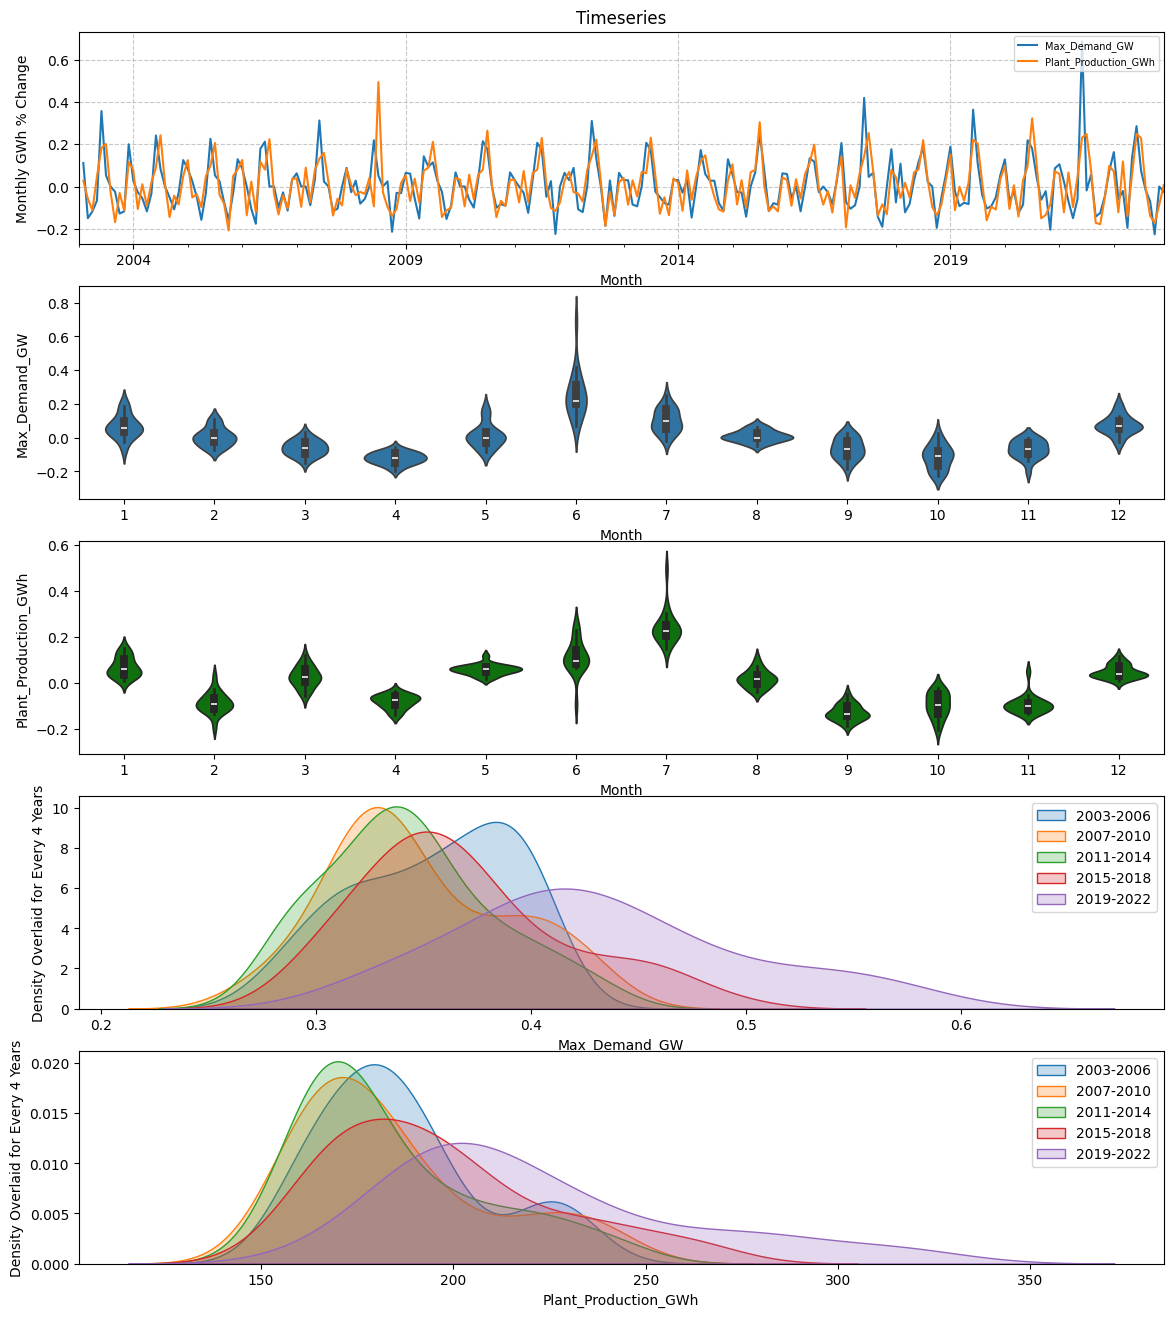
\includegraphics[width=\columnwidth]{data_analysis/production_timeseries.png}
    \caption{Demand and Production Time Series}
    \label{fig:elec_timeseries}
\end{figure}

The GDP was explored in Figure~\ref{fig:gdp_timeseries}. Shifts in the economy can be observed, with larger gains after 2012 (in the first plot). There was an aberration in 2020, probably caused by the COVID pandemic during this time.
\begin{figure}[htb]
    \centering
    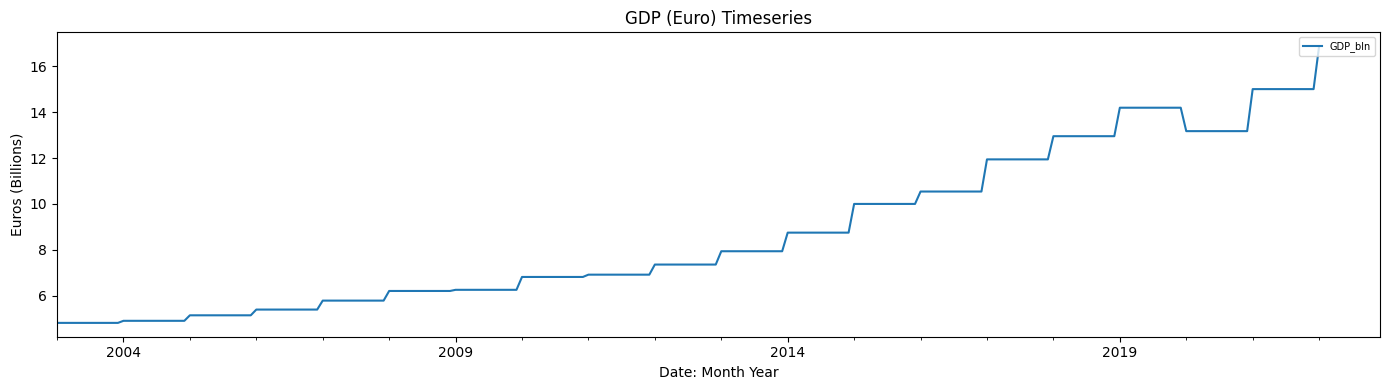
\includegraphics[width=\columnwidth]{data_analysis/gdp_timeseries.png}
    \caption{GDP in Billions of Euros}
    \label{fig:gdp_timeseries}
\end{figure}

Population was explored in Figure~\ref{fig:pop_timeseries}. The population moves with the GDP.
\begin{figure}[htb]
    \centering
    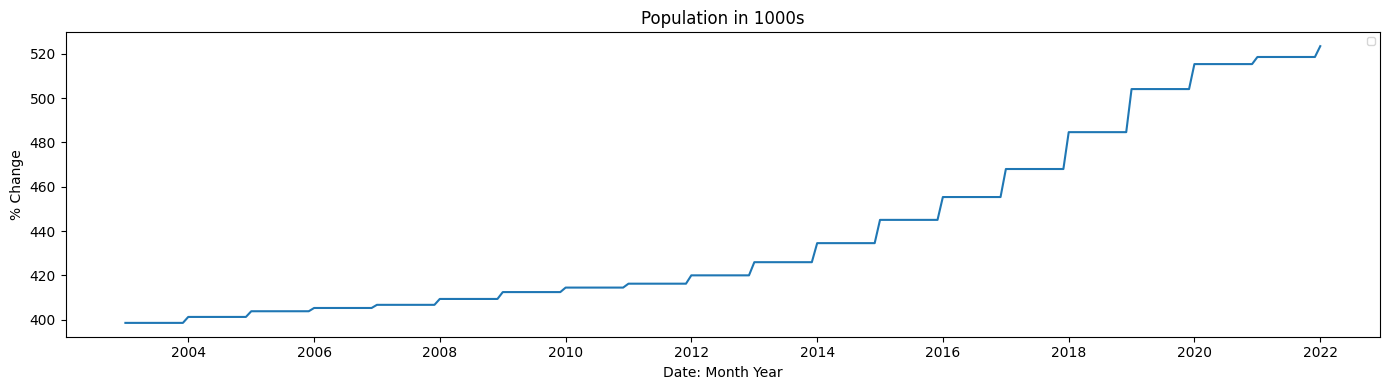
\includegraphics[width=\columnwidth]{data_analysis/population_timeseries.png}
    \caption{Population in 1000s}
    \label{fig:pop_timeseries}
\end{figure}

Finally the climate time series is visualised in Figure~\ref{fig:climate_timeseries}, it has obvious data quality issues in the periodic changes in the first subplot, as shown in the long tailed violin plots. The \textit{prcp}, \textit{wspd} and \textit{pres} parameters were dropped.
In the second subplot, missing or low quality data for \textit{tsun} the Total Sunshine Duration was noted, and to a lesser extend in \textit{tmax} the maximum temperature.
\begin{figure}[htb]
    \centering
    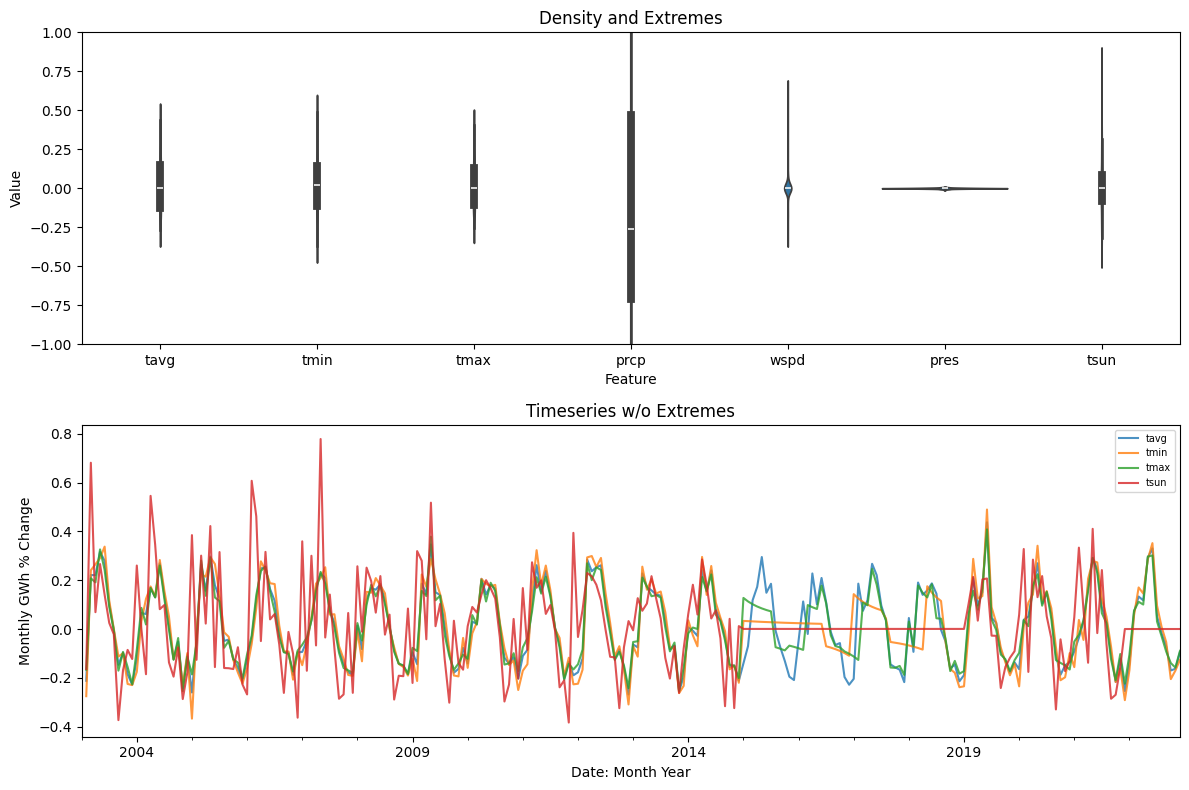
\includegraphics[width=\columnwidth]{data_analysis/climate_timeseries.png}
    \caption{Climate Features}
    \label{fig:climate_timeseries}
\end{figure}

All together, the overlayed time series can be seen in the Figure~\ref{fig:all_timeseries}.
\begin{figure}[htb]
    \centering
    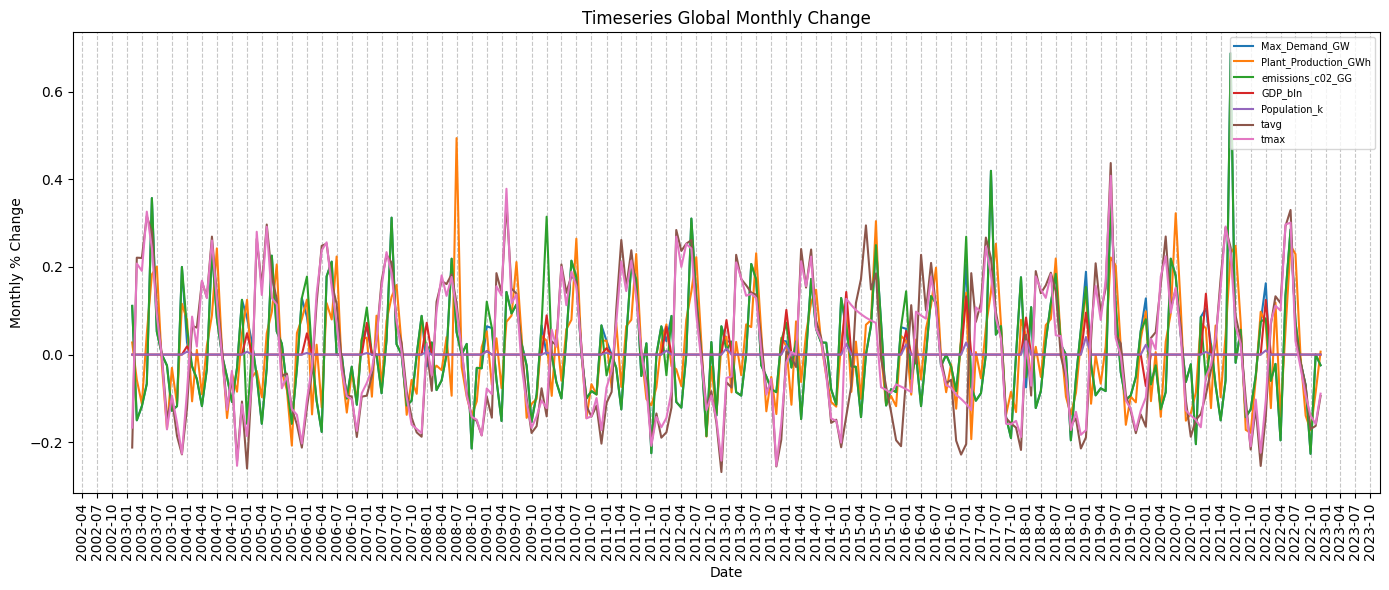
\includegraphics[width=\columnwidth]{data_analysis/all_timeseries.png}
    \caption{All Overlayed Time Series}
    \label{fig:all_timeseries}
\end{figure}

There is correlations that need to be analyzed, and given these are time series data, cointegration can be explored to test if the associations are long term.

We performed pair plots across all features, as shown in Figure~\ref{fig:pair_plots}. The following was observed:
\begin{itemize}
    \item Demand and Production exhibit similar patterns and relationships. Production reflects output over time, whereas demand represents the highest instantaneous output.
    \item The GDP index shows a relationship with both population and emissions, indicating possible multicollinearity. A refinement to GDP per capita is suggested for better analysis.
    \item Climate Data (\textit{tmax} and \textit{tavg}) seem multicollinear though a quadratic relationship with demand exists.
\end{itemize}

\begin{figure}[htb]
    \centering
    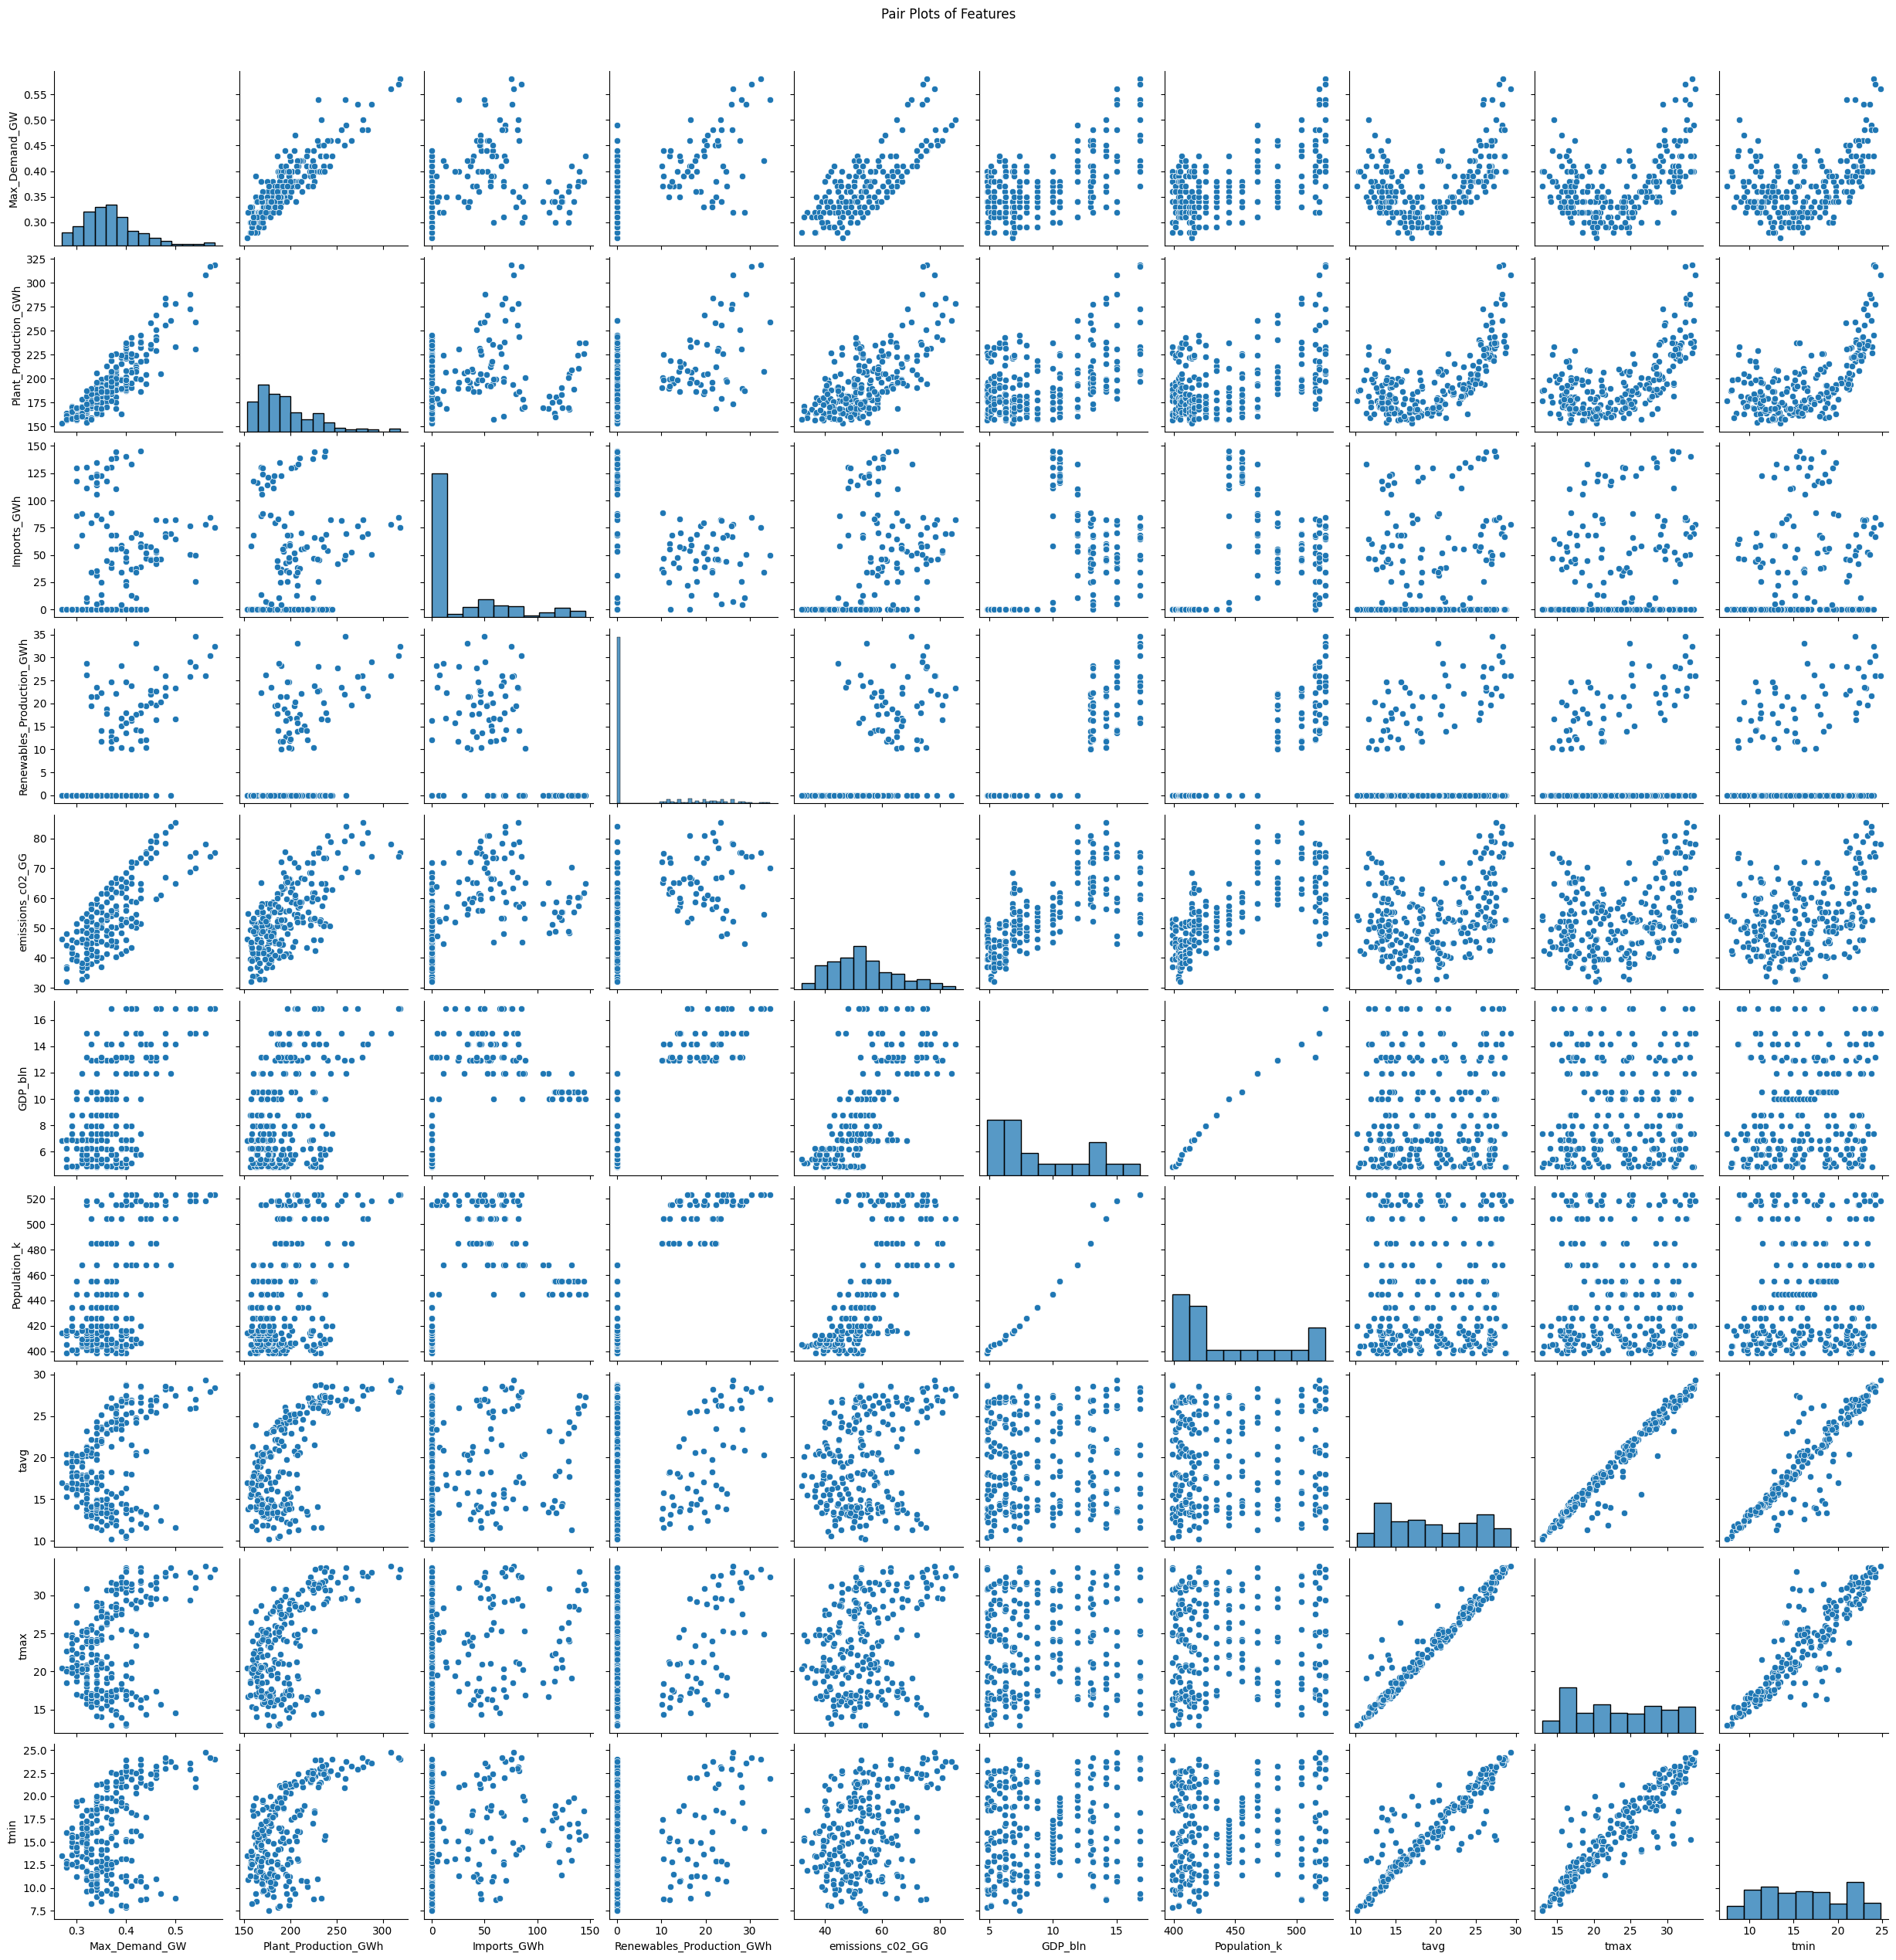
\includegraphics[width=\columnwidth]{data_analysis/pair_plots.png}
    \caption{Pair Plots of all Features}
    \label{fig:pair_plots}
\end{figure}


\subsubsection{Associations and Statistical Tests}
Various associations in the data were explored in Figure~\ref{fig:corr_coint_heatmaps}. This involved statistical tests for correlations and cointegrations at a significance level \(\alpha\) of 0.05 for these two hypothesis:
\begin{enumerate}
    \item \(H0_1\): The features are not correlated, or the correlation is not significant.
    \item \(H0_2\): The time series features are not cointegrated, or the cointegration is not significant.
\end{enumerate}
\begin{figure}[htb]
    \centering
    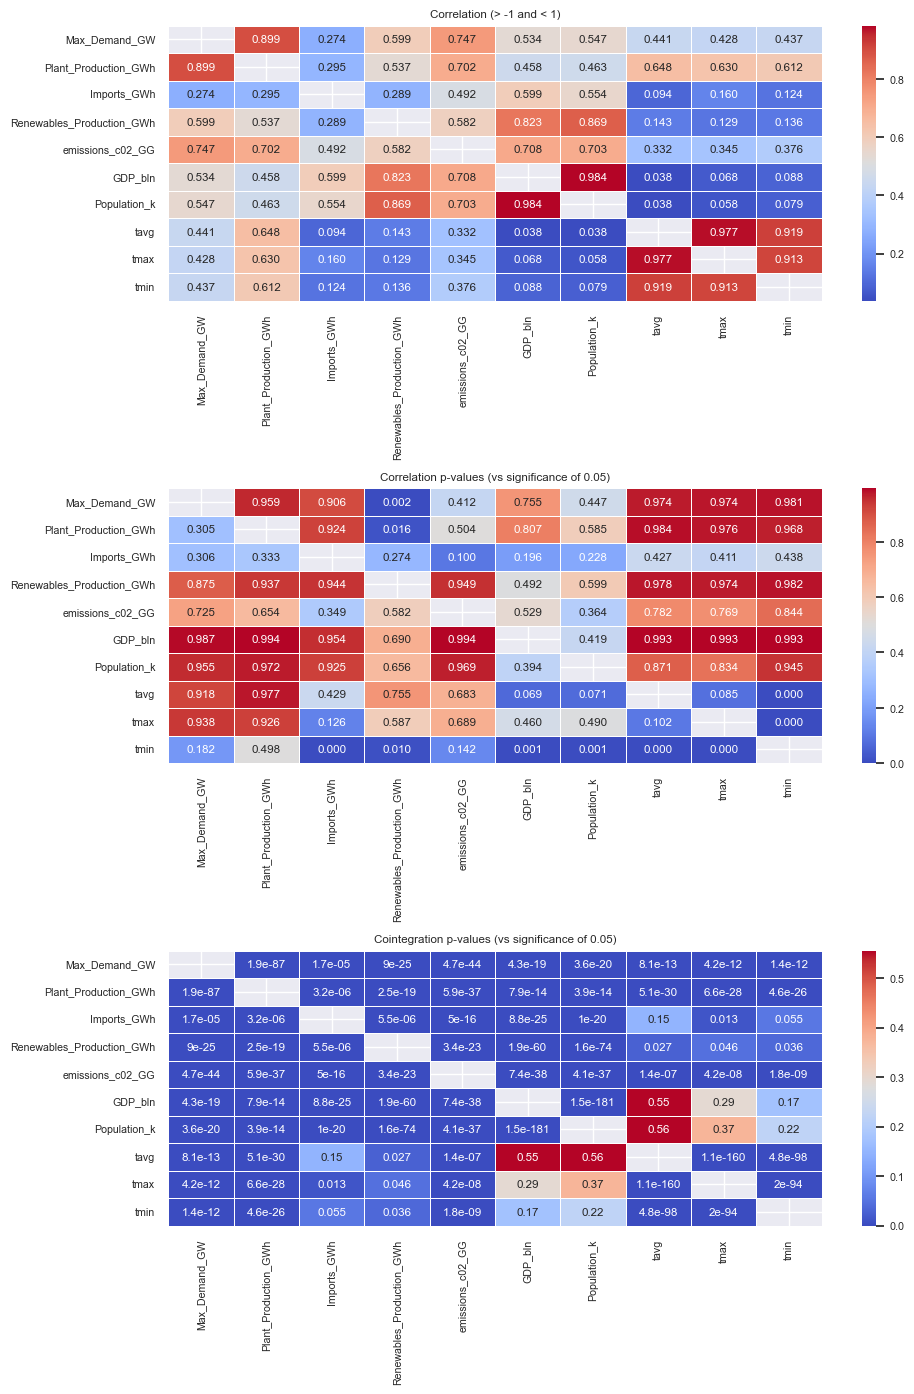
\includegraphics[width=\columnwidth]{data_analysis/corr_coint_heatmap.png}
    \caption{Heatmaps}
    \label{fig:corr_coint_heatmaps}
\end{figure}

The analysis concluded that there was no perceivable cointegration among the features. However, correlations were observed, and there was a high level of confidence in their statistical significance for the following relationships:
\begin{itemize}
    \item Demand and Production: These variables exhibit a strong correlation.
    \item Climate Extremes and Production: The worse the climate conditions, the higher the demand for climate control.
    \item Economic Index and Population: Economic and industrial upticks in Malta led to immigration, resulting in a correlation between economic indicators and population.
    \item CO2 Emissions, Population, and Production.
\end{itemize}

Results of the Hypothesis Tests:
\begin{enumerate}
    \item \(H0_1\) was rejected for features: average temperature, minimum temperature, and maximum temperature, population and GDP. The other correlations may be spurious within our samples.
    \item \(H0_0\) was rejected across all features except with the average temperature with GDP and population, suggesting potential spurious cointegration.
\end{enumerate}

From these tests, the following observations were made:
\begin{itemize}
    \item Average temperature, minimum temperature, and maximum temperature, population and GDP likely exhibit multicollinearity, warranting Variance Inflation Factor (VIF) analysis.
    \item Population and GDP are more accurately represented using GDP per capita.
    \item Strong cointegration indicates a common long-term trend and mutual influence among features.
    \item Features with strong cointegration but without strong correlation, may imply external factors in affect which we aren't capturing.
    \item Asymmetric p-values between demand and production suggest a directional relationship, with maximum demand influencing electricity production, but not vice versa.
\end{itemize}

Given the high probability of multicollinearity, we tested the data with VIF and a constant, achieving the results in Table~\ref{cointTable}.
\begin{table}[h!]

\centering
\caption{Variance Inflation Factors for each feature}
\begin{tabular}{|l|c|}
\hline
\textbf{Feature} & \textbf{VIF} \\
\hline
const & 3874.53 \\
Plant\_Production\_GWh & 3.83 \\
Imports\_GWh & 2.17 \\
Renewables\_Production\_GWh & 7.20 \\
emissions\_c02\_GG & 3.56 \\
GDP\_bln & 41.07 \\
Population\_k & 52.91 \\
tavg & 30.21 \\
tmax & 26.01 \\
tmin & 7.05 \\
\hline
\end{tabular}
\label{cointTable}
\end{table}

Given all the tests above, it was concluded that the best features to use to predict \textit{Electricity Demand} are:
\begin{itemize}
    \item Plant Production
    \item CO2 emissions
    \item Average Temperature
    \item GDP (or the GDP per capita proxy including population)
\end{itemize}

\subsubsection{Time Series Tests}
A time series $Y$ is comprised of four components: $Y(t)=T(t)S(t)C(t)\epsilon(t)$, where $T$ is the trend, $S$ is the seasonal trend, $C$ is the cyclical trend and $\epsilon$ is noise in any point at time $t$.
The component $Y$ can be predicted with historical data, if the time series is Auto Regressive (AR), which can be tested for using the auto correlation function, which measures the linear predictability of target variable using adjacent points in two time series. From Figure~\ref{fig:acf1} autoregression (AR) is observed at lags 1, 2, 11, 12, with a Pearson correlation of 0.6 to 0.8, indicating the AR nature of the dataset.
\begin{figure}[htb]
    \centering
    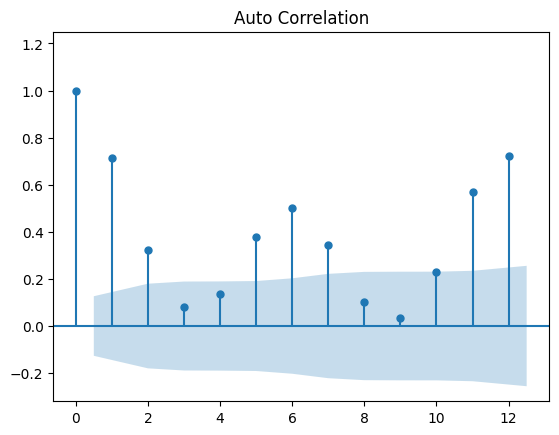
\includegraphics[width=\columnwidth]{data_analysis/acf1.png}
    \caption{Autregression Lags}
    \label{fig:acf1}
\end{figure}
Seasonality is apparent in the time series, and this was further tested with \textit{Seasonal Decomposition}($T$, $S$, and $C$ weights through time) to check for non-stationarity, as shown in Figure~\ref{fig:acf3}.

\begin{figure}[htb]
    \centering
    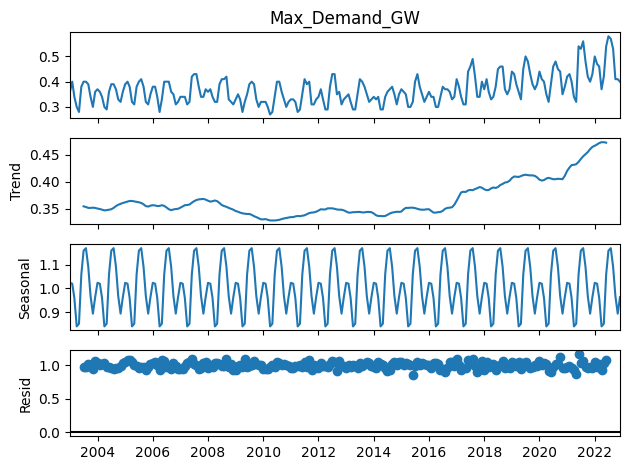
\includegraphics[width=\columnwidth]{data_analysis/acf3.png}
    \caption{Time Series Decomposition (Multiplicative)}
    \label{fig:acf3}
\end{figure}

Finally, we test the null hypothesis \(H0\) that the data is not stationary, using an Augmented Dickey–Fuller test. If the T-statistic and P-value are large: \(H0\) is not rejected, indicating non-stationarity and the presence of a unit root. For stationarity, $\text{P-value} \leq \text{significance level}, \quad \text{T-stat} \leq \text{critical value}$ see Table~\ref{adfTable} and Table~\ref{adfTableCrit}.

\begin{table}[h!]

\centering
\caption{Augmented Dickey–Fuller Test Results}
\begin{tabular}{|l|c|}
\hline
\textbf{Metric} & \textbf{Value} \\
\hline
T-stat & 0.212656 \\
p-value & 0.972963 \\
\hline
\end{tabular}

\label{adfTable}
\end{table}

\begin{table}[h!]

\centering
\caption{Critical Values for Augmented Dickey–Fuller Test}
\begin{tabular}{|l|c|}
\hline
\textbf{Critical Value Level} & \textbf{Value} \\
\hline
1\% & -3.459884913337196 \\
5\% & -2.8745310704320794 \\
10\% & -2.573693840082908 \\
\hline
\end{tabular}

\label{adfTableCrit}
\end{table}


\section{Data Reduction Techniques}
The following section describes the data reduction techniques employed to facilitate the construction of the algorithms.

\subsection{Principal Component Analysis}

Principal Component Analysis (PCA) performed on the dataset provided insight on how much information the individual features contribute. The steps taken for PCA are detailed below..

\begin{enumerate}

\item Data was normalised, all our features $\mathbf{X}$ were centered and scaled by subtracting the mean $\boldsymbol{\mu}$ and dividing by the standard deviation $\boldsymbol{\sigma}$. This normalisation uses the transformation~\ref{normEq}.
\begin{equation}
\mathbf{z} = \frac{\mathbf{x} - \boldsymbol{\mu}}{\boldsymbol{\sigma}}
\label{normEq}
\end{equation}

\item A covariance matrix was calculated for the feature set, where $\text{Cov(X)}$ is a matrix of scaled features $X$ that captures most movements between each pair of features,  \( \overline{X} \) is the mean feature vector, computed across samples, and given by Equation~\ref{covEq}.

\begin{equation} \label{covEq}
\text{Cov(X)} = \frac{1}{n-1}(X - \overline{X})' \cdot (X - \overline{X})
\end{equation}

\item Eigen Decomposition was performed to reduce Cov(x) to its constituent parts by solving for the eigenvectors \( \mathbf{V} \) and eigenvalues \( \boldsymbol{\lambda} \). An eigenvector \( \mathbf{v}_i \) changes by multiplying the eigenvalue \( \lambda_i \) scalar, the magnitude of this change is the information that component holds.

\item Finally the variance was explained by each principal component calculated. The top five components explained 95\% of the variance in Figure~\ref{fig:variance}

\end{enumerate}

\begin{figure}[htb]
    \centering
    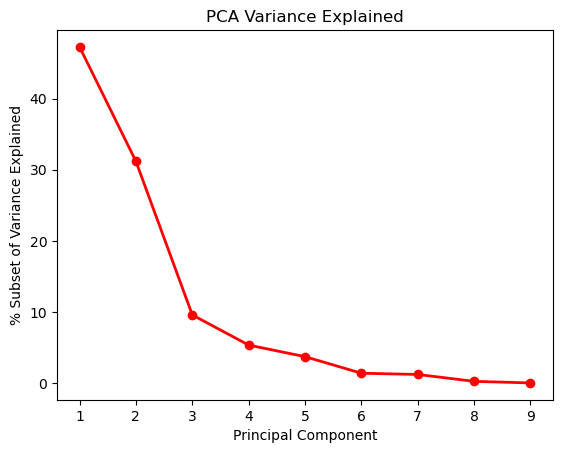
\includegraphics[width=0.45\textwidth]{DIM-PCA/variance_explained.png}
    \caption{Cumulative Variance Explained}
    \label{fig:variance}
\end{figure}

In Figure~\ref{fig:loadings}, the feature loadings show the correlation between original features and the principal components.

\begin{figure}[htb]
    \centering
    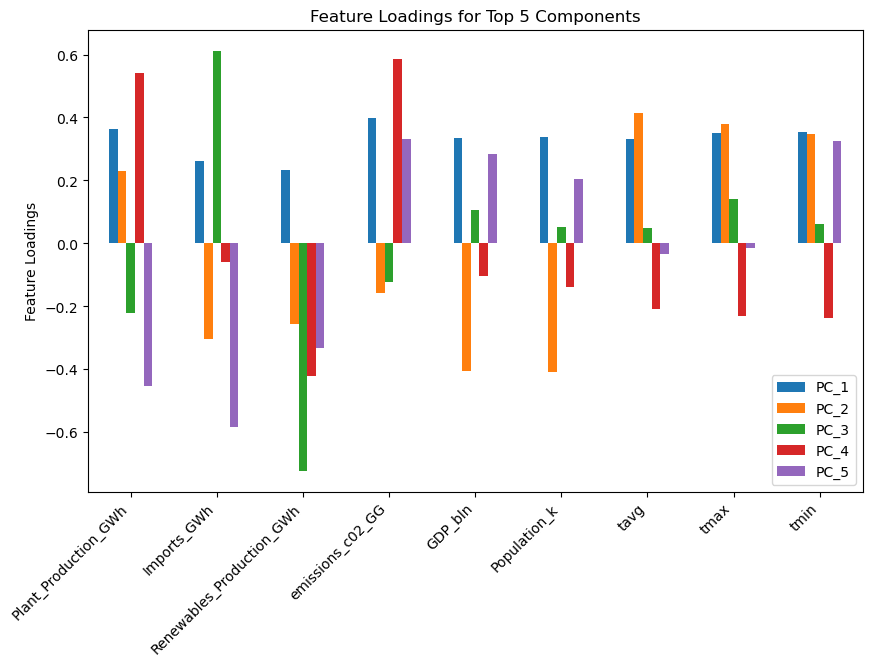
\includegraphics[width=0.45\textwidth]{DIM-PCA/feature_loadings.png}
\caption{Feature Loadings}
    \label{fig:loadings}
\end{figure}

Aggregating the absolute loading for each feature, the most relevant features in our dataset are ranked in Table~\ref{tab:PCA}.

\begin{table*}[!t]
\caption{Principal Component Analysis Results for Five Components}
\centering
\begin{tabular}{|l|c|c|c|c|c|}
\hline
& \textbf{PC\_1} & \textbf{PC\_2} & \textbf{PC\_3} & \textbf{PC\_4} & \textbf{PC\_5} \\
\hline
Plant\_Production\_GWh & 0.364894 & 0.229681 & -0.222024 & 0.540538 & -0.453880 \\
Imports\_GWh & 0.260468 & -0.302942 & 0.612521 & -0.059604 & -0.584167 \\
Renewables\_Production\_GWh & 0.234642 & -0.257417 & -0.722040 & -0.419919 & -0.333823 \\
emissions\_c02\_GG & 0.397053 & -0.158149 & -0.121997 & 0.587074 & 0.332110 \\
GDP\_bln & 0.335650 & -0.404069 & 0.104817 & -0.104691 & 0.284875 \\
Population\_k & 0.339181 & -0.408691 & 0.050466 & -0.137694 & 0.205907 \\
tavg & 0.332240 & 0.413588 & 0.048856 & -0.209620 & -0.034683 \\
tmax & 0.350576 & 0.377868 & 0.140084 & -0.231299 & -0.014188 \\
tmin & 0.353990 & 0.346496 & 0.061280 & -0.236471 & 0.325653 \\
\hline
\end{tabular}

\label{tab:PCA}
\end{table*}

The top five features validated here are:

\begin{itemize}
    \item Plant Production
    \item Emissions
    \item GDP
    \item Temperature
    \item Population (Colinear with GDP).
\end{itemize}

Although PCA can hint on the important features in the data, it has known pitfalls with a time series which is non-stationary as the mean and variance moves \cite{pca_ts_paper}.

\section{Experiments}

The following sub-sections detail the experiments carried out to implement the various algorithms selected, as explained in Section~\ref{sec:background}. The TCN algorithm was implemented using TensorFlow, while the rest were implemented using Sci-Kit Learn models.

\subsection{Temporal Convolution Networks} \label{TCNarch}

In this experiment, a Temporal Convolution Network (TCN) was built in TensorFlow2. To test and validate the TCN, an AutoARIMA model acted as a baseline. Both models predicted the next month's maximum power demand. As both are AR models, the target label was also included as a feature to the models.

\subsubsection{Baseline AutoARIMA Model}

ARIMA stands for AutoRegressive Integrated Moving Average model. An ARIMA model predicts \( \hat{y}(t) \) through:
\begin{equation}
\hat{y}(t) = \alpha_1 \cdot Y(t-1)
\label{eq:arima}
\end{equation}
as described in \cite{Zhang2018}. Where $\alpha_1$ is the parameter that the AutoARIMA model will select, and $Y(t-1)$ is the previous value.

The construction of a baseline ARIMA model is out of scope for this experiment, and an AutoARIMA model was used to select an adequate model without further fine-tuning.

\subsubsection{Temporal Convolution Network Architecture}

The TCN architecture followed the designs of Gasparin, Alberto, Slobodan Lukovic, and Cesare Alippi (2020)~\cite{Gasparin2022}. Their convolution network's operations over consecutive layers can be represented with the following Equation~\ref{tcnEq}:
\begin{equation} \label{tcnEq}
x_{l}^{t} = g\left(\sum_{k=0}^{K-1} w_{lk} \cdot x_{l-1}^{t-(k \times d)} + b_l\right)
\end{equation}
Where:
\begin{itemize}
    \item \( x_{l}^{t} \) is the output of the neuron at position \( t \) in the \( l \)-th layer.
    \item \( K \) is the kernel's with, determining the number of past time windows considered.
    \item \( w_{lk} \) is the weight for the \( k \)-th position in the kernel used to give importance to past data.
    \item \( d \) is the dilation factor, or the space between inputs allowing the network to integrate historical information.
    \item \( b_l \) is the bias term.
    \item \( g \) is ReLU defined as \( g(x) = \max(0, x) \).
\end{itemize}

The architecture built can be visualised in Figure~\ref{fig:TCN_architecture_graph}.

% \begin{figure}[htb]
%     \centering
%     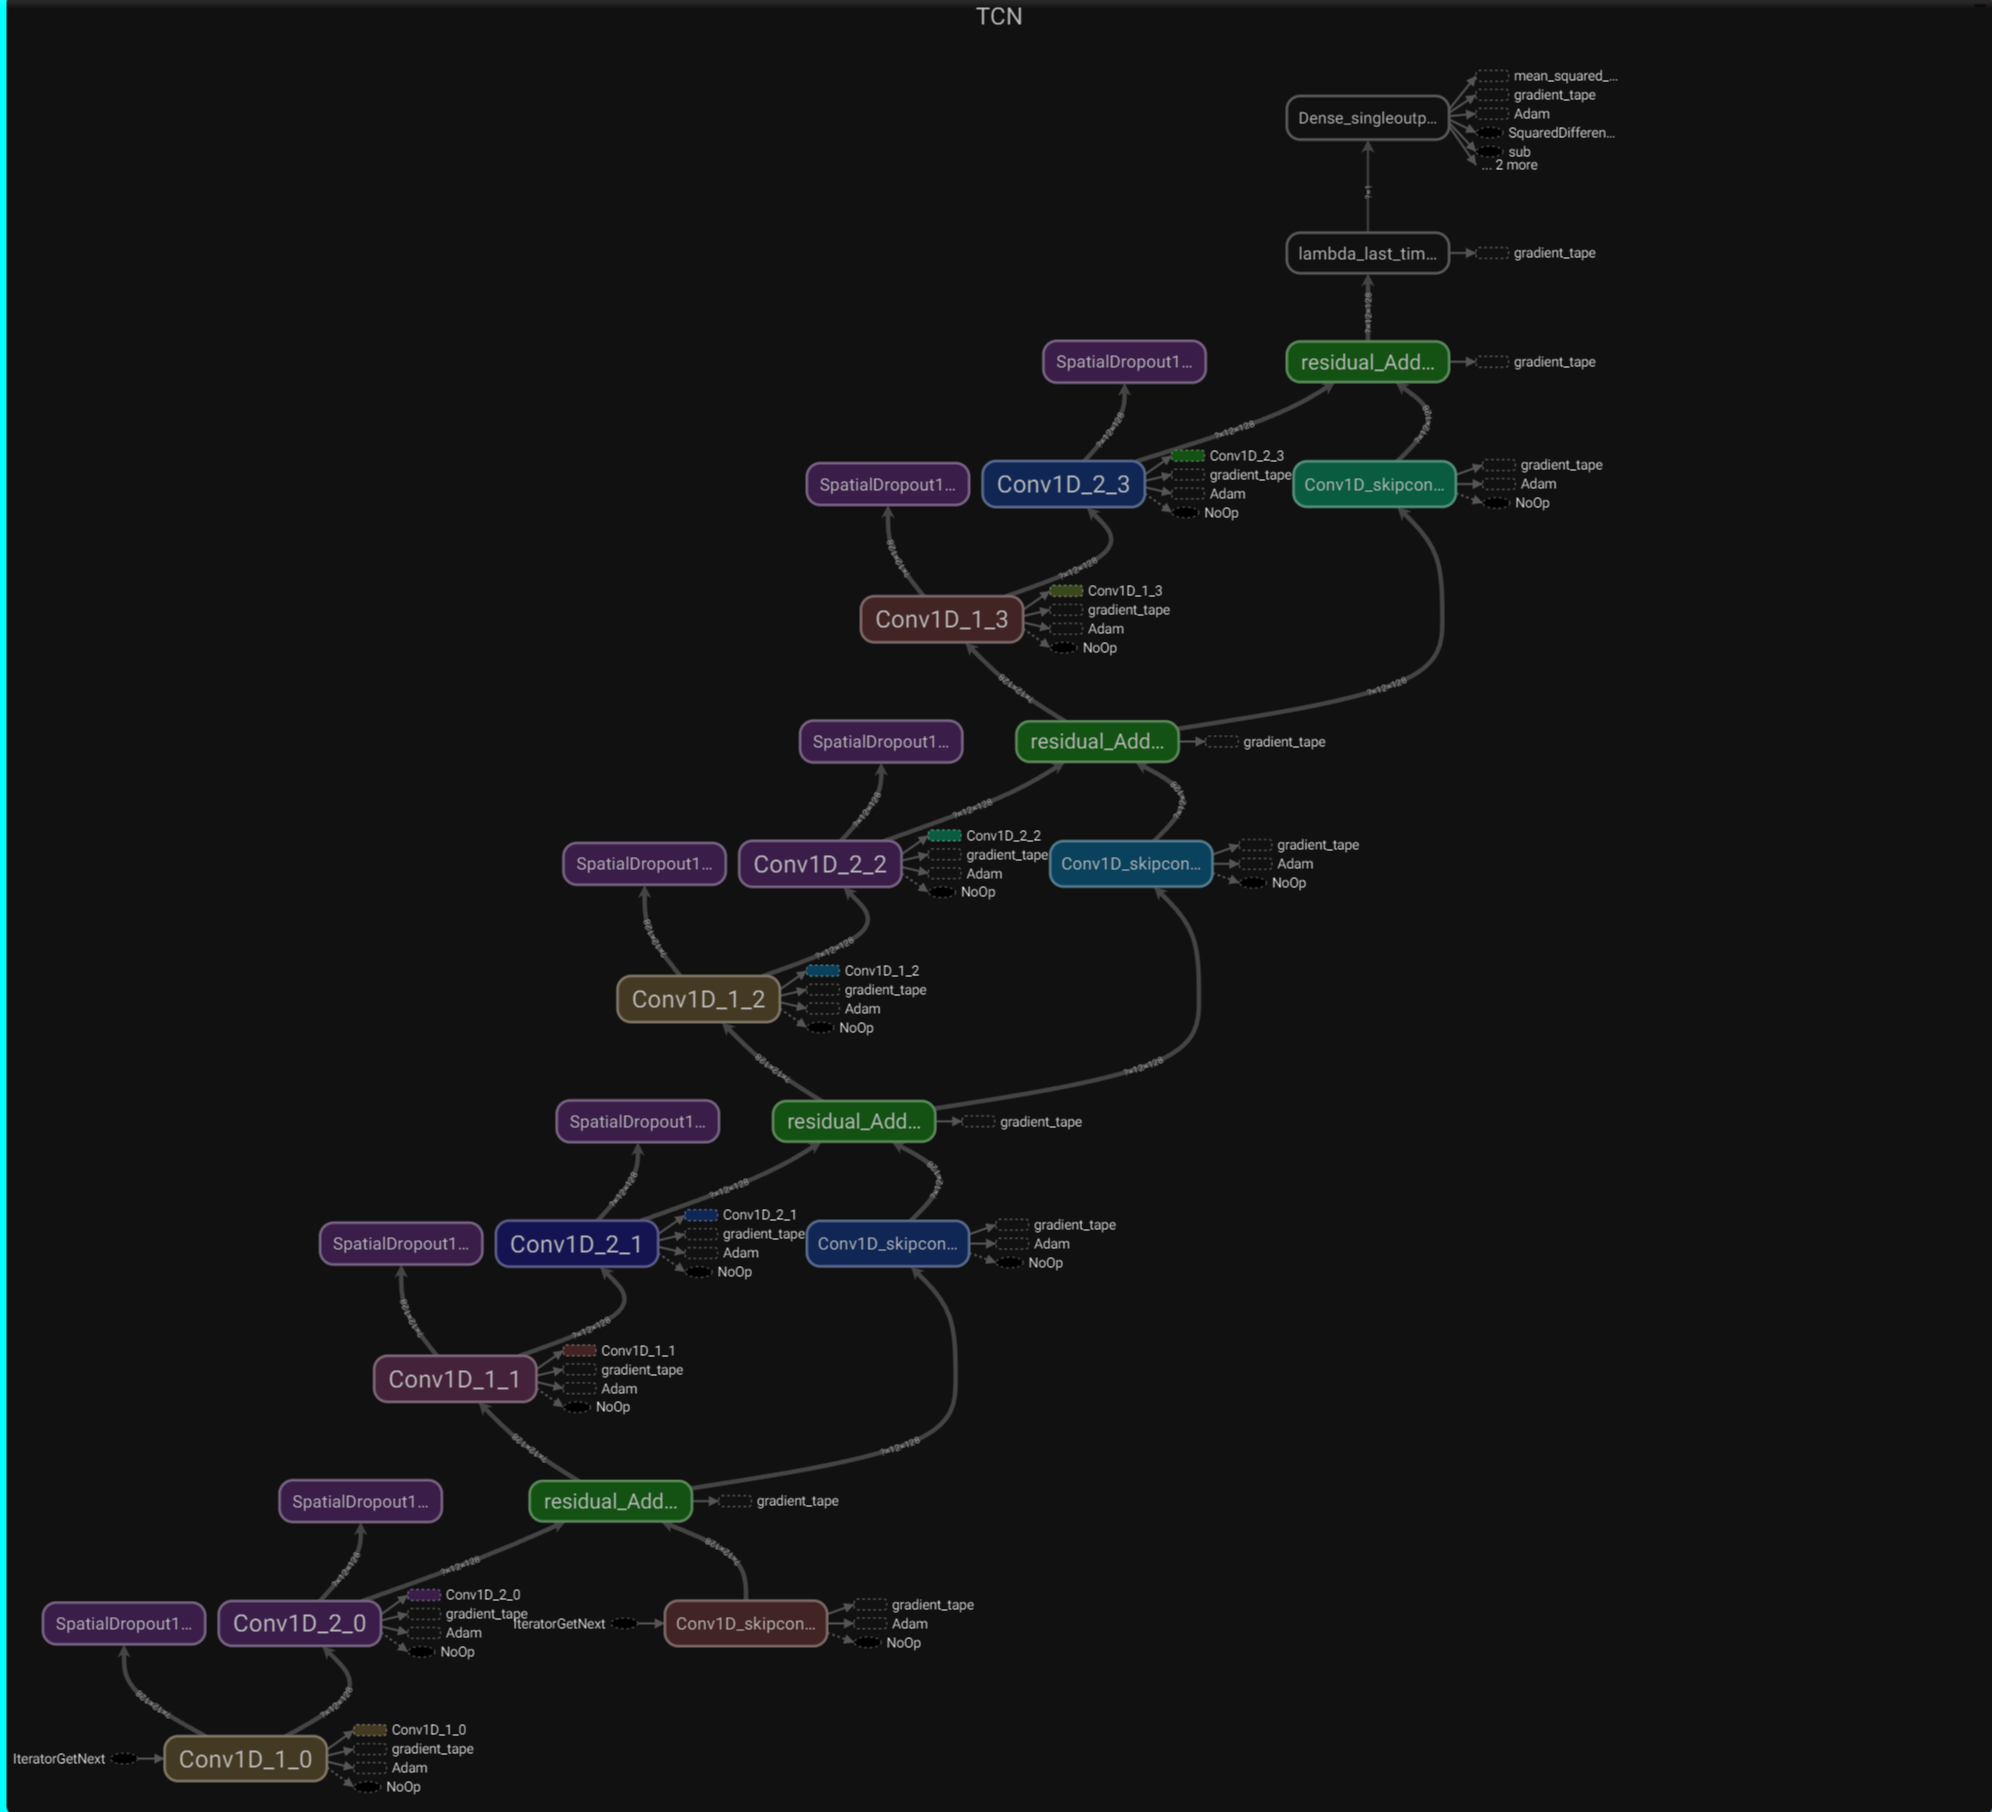
\includegraphics[width=\columnwidth]{Model-TCN/TCN_architecture_graph.PNG}
%     \caption{TCN Architecture}
%     \label{fig:TCN_architecture_graph}
% \end{figure}

\subsubsection{Encoding Time Windows}

The data was normalised and encoded into year-long windows, with a one-month lag from the ACF results.  The dates themselves were engineered as a new feature in the form of sine and cosine waves to capture the cyclic nature of date-time features.

\subsubsection{Dilated Causal Convolutions}
The dilation factor in the TCN increases exponentially with the depth of the network, allowing the neurons to capture history, without leakage.

\subsubsection{Grid Search}

hyper-parameters were inferred through a grid search method. The grid search ran for 3 days on an 8core 3.60GHz Intel CPU with 16GB RAM.

The tested parameters were chosen from Benitez et al. (2020) with minor additions~\cite{Benitez2020}. The grid search results are available in Table~\ref{tab:hyperparameters}.

\begin{table}[h]
\centering
\caption{Hyper-parameter Grid and Selected Values}
\begin{tabular}{lcc}
\hline
Hyper-parameter & Grid Values & Selected Value \\
\hline
Number of Filters & 32, 64, 128 & 128 \\
Kernel Size & 2, 3, 4 & 4 \\
Batch Size & 64, 128, 256 & 32 \\
Epochs & 25, 50, 100, 300 & 300 \\
Dilation Rate & 1, 2, 4 & 4 \\
Dropout Rate & 0.1, 0.2, 0.3 & 0.5 \\
Number of Layers & 6, 5, 4, 3 & 4 \\
L2 Regularization & 0.005, 0.001, 0.01 & 0.005 \\
Learning Rate & 0.001, 0.01, 0.1 & 0.0001 \\
\hline
\end{tabular}
\label{tab:hyperparameters}
\end{table}

\subsubsection{Experiment Results}

The error results of the TCN vs the baseline AutoARIMA are visible in Table~\ref{tab:metrics_comparison}
\begin{table}[h]
\centering
\caption{TCN vs AutoARIMA Baseline}
\begin{tabular}{lccc}
\hline
Metric & AutoARIMA & TCN & TCN Outperforms? \\
\hline
MAE & 0.036 & 0.035 & Yes \\
MAPE & 	7.75\% & 7.83\% & No \\
MSE & 0.0023 & 0.0021 & Yes \\
R2 & 0.46 & 0.51 & Yes \\
RMSE & 0.048 & 0.046 & Yes \\
SMAPE & 8.22\% & 8.13\% & Yes \\
WAPE & 8.36\% & 7.47\% & Yes \\
\hline
\end{tabular}
\label{tab:metrics_comparison}
\end{table}

As expected, the TCN outperforms on every metric but MAPE. The TCN probably performed well on most data but poorly on a few data points, as MAPE is a relative error measure. MAPE might not be the best metric for this problem, it is known to have issues with very low values~\cite{scikitMAPE}.

Visually, Figure~\ref{fig:tcnpredictions} shows how the TCN can capture trends and latent relationships in the data, compared to the baseline ARIMA model.
\begin{figure}[htb]
    \centering
    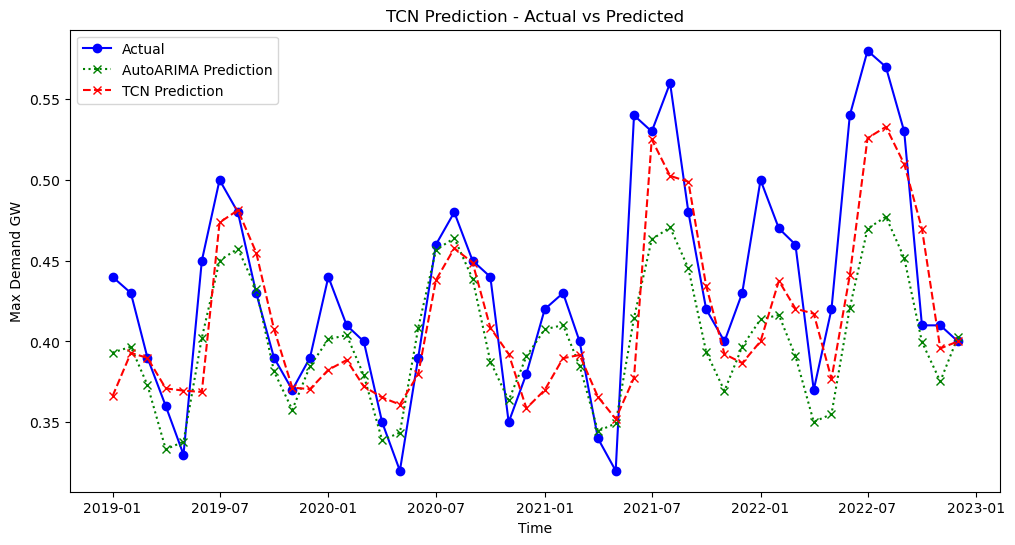
\includegraphics[width=\columnwidth]{Model-TCN/TCN_Actual_Vs_predicted.png}
    \caption{The TCN's predictions against the actual and baseline model.}
    \label{fig:tcnpredictions}
\end{figure}

\section{Discussion}
A thorough evaluation was conducted, metrics below.


\section{Conclusion}
In this research, we have successfully answered our research question.

\newpage
\begin{thebibliography}{00}

\bibitem{Zhang2018}Zhang, Mingda. "Time series: Autoregressive models ar, ma, arma, arima." University of Pittsburgh (2018).

\bibitem{Gasparin2022}Gasparin, Alberto, Slobodan Lukovic, and Cesare Alippi. "\emph{Deep learning for time series forecasting: The electric load case.}" CAAI Transactions on Intelligence Technology 7.1 (2022): 1-25.

\bibitem{Benitez2020}Lara-Benítez, Pedro, et al. "Temporal convolutional networks applied to energy-related time series forecasting." applied sciences 10.7 (2020): 2322.

\bibitem{SVR_Electricity_consumption} Duan J, Tian X, Ma W, Qiu X, Wang P, An L. \emph{Electricity Consumption Forecasting using Support Vector Regression with the Mixture Maximum Correntropy Criterion. Entropy (Basel). 2019 Jul 19;21(7):707. doi: 10.3390/e21070707. PMID: 33267421; PMCID: PMC7515222. }\url{https://www.ncbi.nlm.nih.gov/pmc/articles/PMC7515222/}

\bibitem{elec_supp_src} National Statistics Office, \emph{Electricity Supply: 2022} \url{https://nso.gov.mt/electricity-supply-2022/?fbclid=IwAR3ZCJBJjgVKAS6MyXQR__Rhg3zEaJQXsG1Nz-1IYWDCtezH3N26rIdL3ZA}

\bibitem{elec_gen_statista_src} Eurostat \emph{Net electricity generation by type of fuel - monthly data} \url{https://ec.europa.eu/eurostat/databrowser/view/nrg_cb_pem__custom_8232363/default/table?lang=en}

\bibitem{emmisions_src} Malta Resources Authority, \emph{Total Emissions by Sector} \url{https://public.tableau.com/app/profile/maltaresourcesauthority/viz/test_16911097613970/BySector}

\bibitem{meteostat_api} Meteostat Developers \url{https://public.tableau.com/app/profile/maltaresourcesauthority/viz/test_16911097613970/BySector}

\bibitem{eu_climate_src} European data, \url{https://data.europa.eu/enr}

\bibitem{gdp_src} The World Data Bank, \emph{GDP: linked series (current LCU) - Malta} \url{https://data.worldbank.org/indicator/NY.GDP.MKTP.CN.AD?locations=MT&view=chart}

\bibitem{resample_src} Pandas PyData \emph{pandas.DataFrame.resample} \url{https://pandas.pydata.org/docs/reference/api/pandas.DataFrame.resample.html}

\bibitem{scalar} scikit-learn.org \emph{sklearn.preprocessing.StandardScaler} \url{https://scikit-learn.org/stable/modules/generated/sklearn.preprocessing.StandardScaler.html}

\bibitem{pca_ts_paper} Hamilton, J. D., \& Xi, J. (2022). \emph{Principal Component Analysis for Nonstationary Series}. University of California at San Diego. May 28, 2022. Revised: January 13, 2023. \url{https://econweb.ucsd.edu/~jhamilto/HX.pdf}

\bibitem{scikitMAPE} Scikit-Learn Developers. (2023). \texttt{sklearn.metrics.mean} \texttt{\_absolute\_percentage\_error}. Retrieved December 1, 2023, from \url{https://scikit-learn.org/stable/modules/generated/sklearn.metrics.mean\_absolute\_percentage\_error.html}

\end{thebibliography}

\newpage
\begin{figure}[htb]
    \centering
    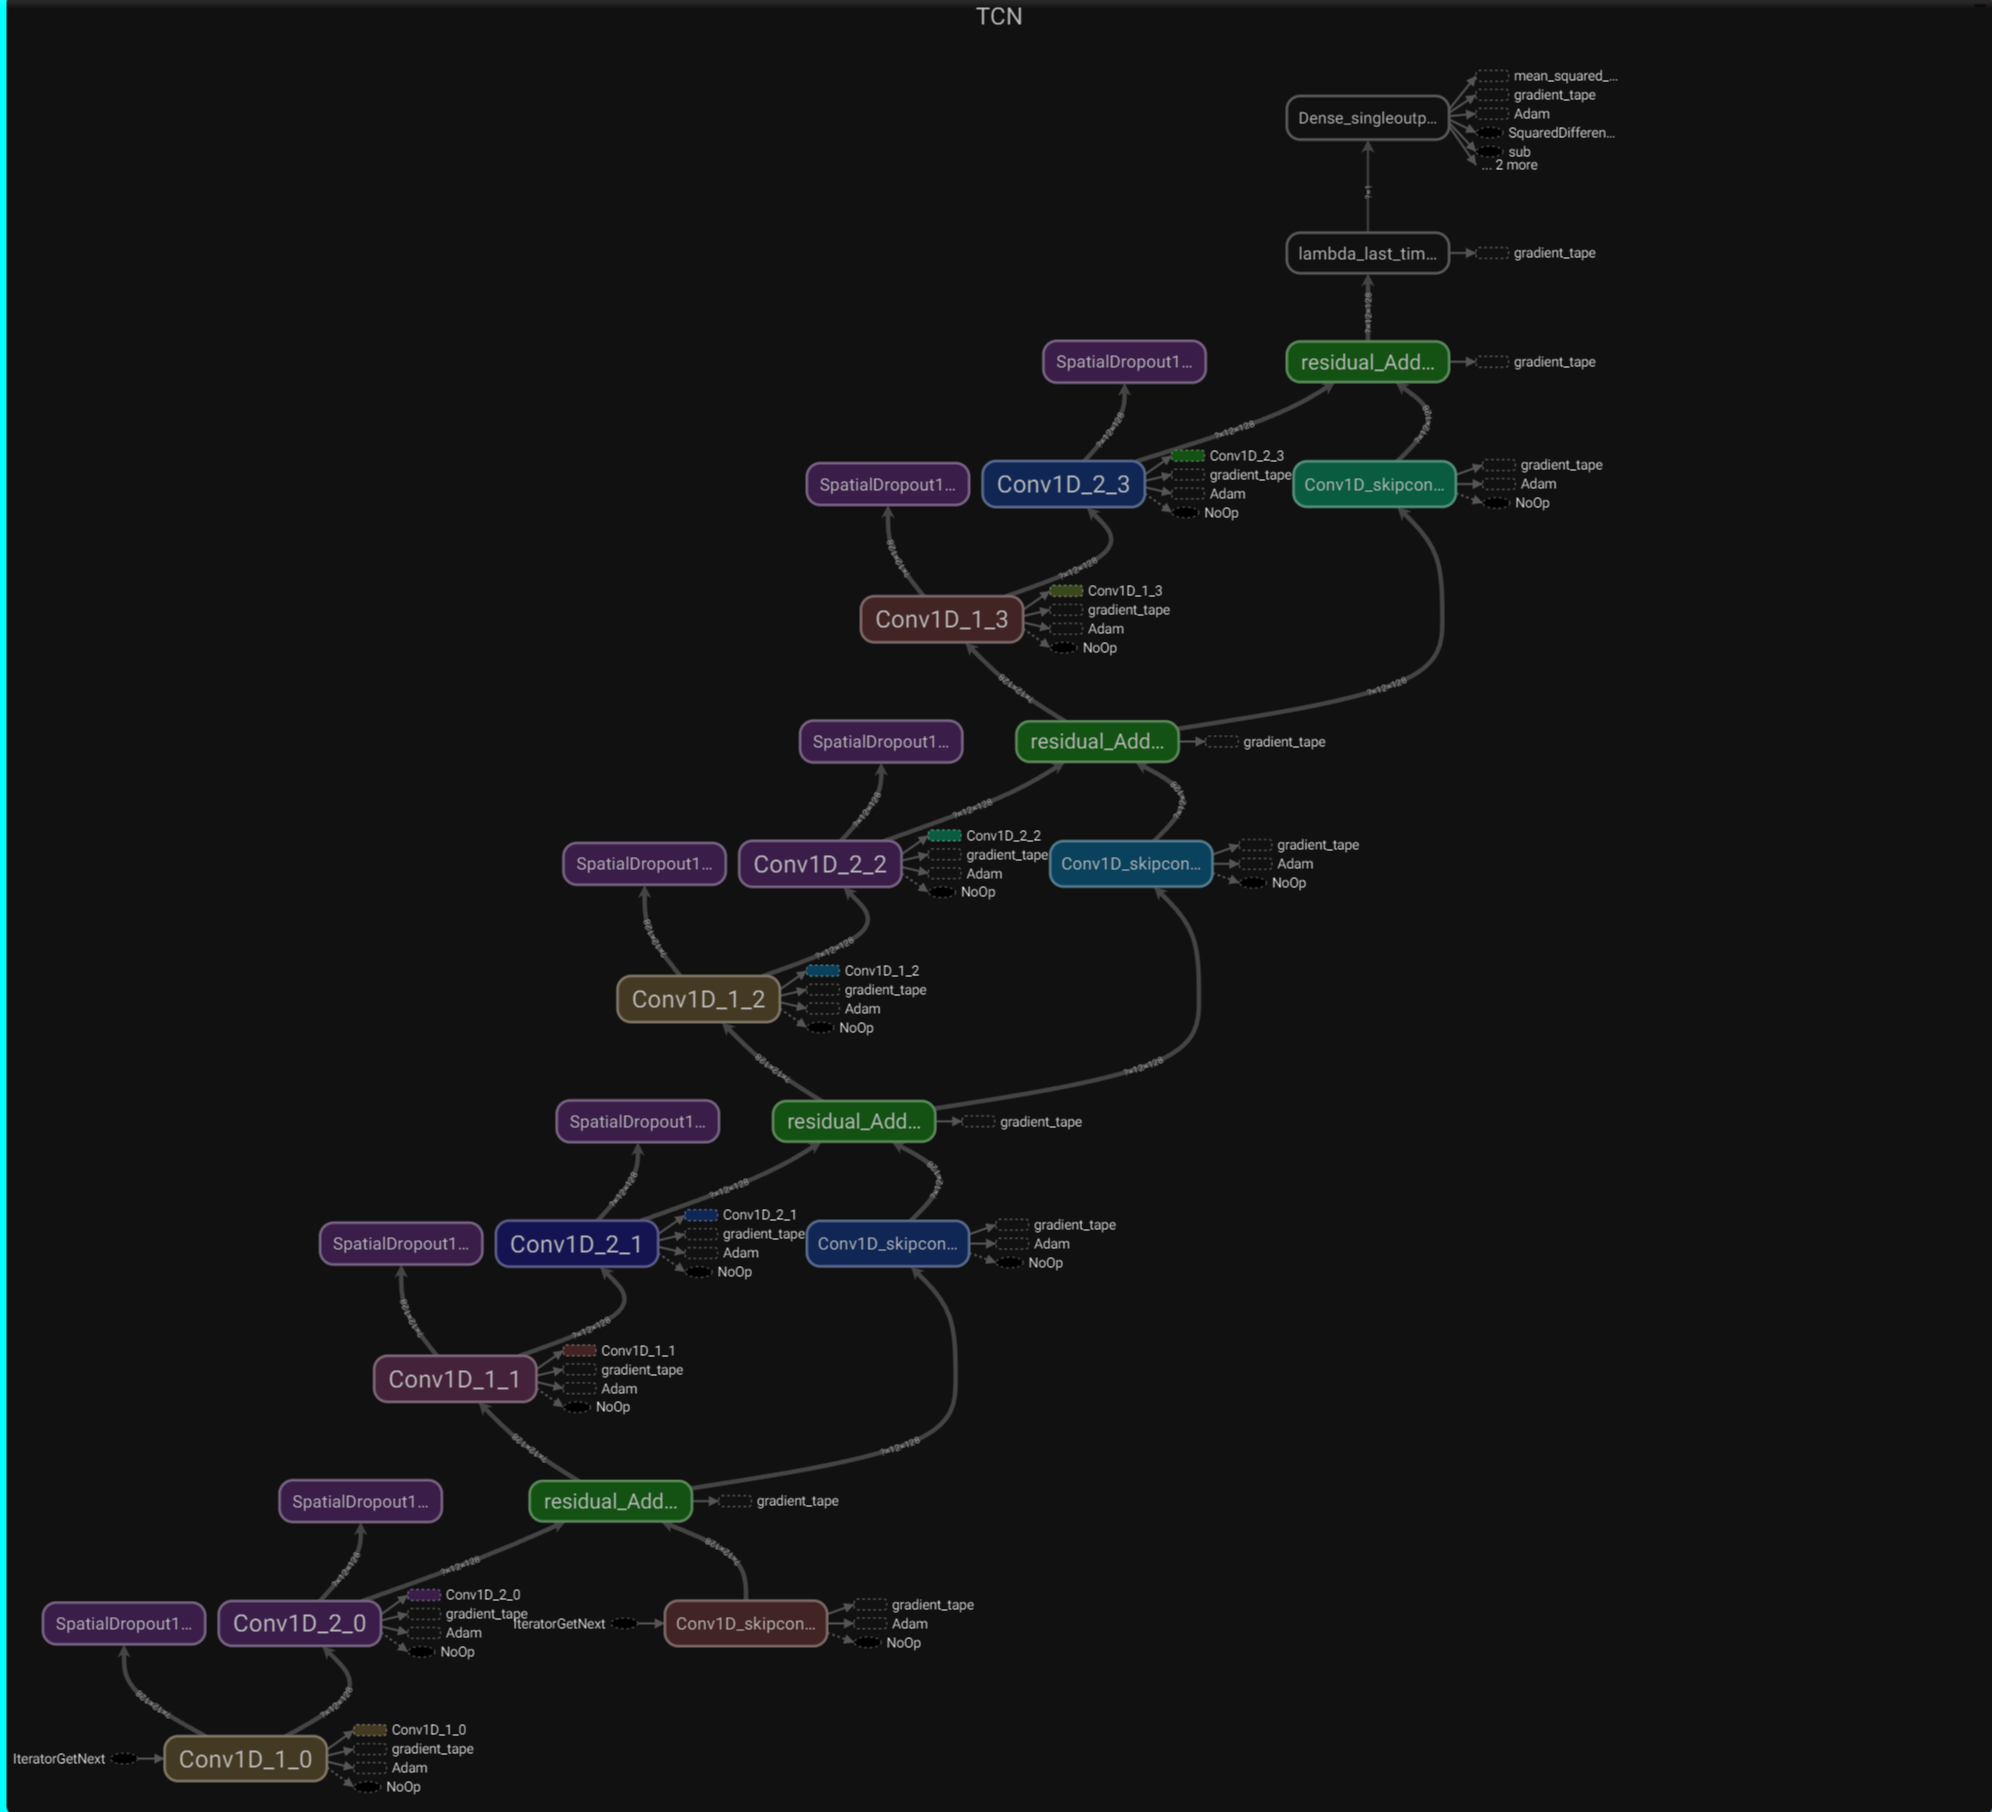
\includegraphics[width=2\columnwidth]{Model-TCN/TCN_architecture_graph.PNG}
    \caption{TCN Architecture}
    \label{fig:TCN_architecture_graph}
\end{figure}

\EOD

\end{document}